\section{World Wide Web Service}
\label{sec:web}

\subsection{Design}

A World Wide Web (WWW) service\citep{rfc1630}\citep{rfc2616} in the network allows any terminal devices to access the deployed webpages. The service in BT Network is established after routers and three laptops have been configurated and DNS service been set up.

For this lab, \texttt{apache2} package is chosen as the tool to establish the web server on Laptop 1 (BT001). 
Using the default settings of this package is enough and it has a specific folder static web pages are stored. 


\subsection{Implementation}

Install \texttt{apache2} package on Laptop 1 (BT001, IPv4 Address: 23.0.0.2) using following the command.

\begin{lstlisting}[language=sh]
sudo apt-get install apache2
\end{lstlisting}

A HTML file named \texttt{index.html} is created as a test webpage, as detailed in Figure \ref{fig:index-html}.

\begin{figure*}[ht!]
\begin{lstlisting}[language=html]
<html>
<header><title>BT Network</title></header>
<body>
<h1>Welcome to BT Network |</h1>
A Trustworthy Internet Service Provider at Loughborough University.
</body>
</html>
\end{lstlisting}
\caption{Contents of HTML File Named \texttt{index.html}}
\label{fig:index-html}
\end{figure*}

Then, the HTML file is copied to the folder \texttt{/var/www/html}. This folder is used to deploy webpages on the server. And the meaning of ‘-r’ is to cover the same name file. 

\begin{lstlisting}[language=sh]
cp -r index.html /var/www/html
\end{lstlisting}

Then, install \texttt{links} package which is a command-line Web browser in Linux by using following command.

\begin{lstlisting}[language=sh]
sudo apt-get install links
\end{lstlisting}


Then, \texttt{links} is started and the web page is accessed through URL with the local IP address.

\begin{lstlisting}[language=sh]
links http://23.0.0.2/
\end{lstlisting}

Finally, add the following lines to the forward DNS file \texttt{/etc/bind/db.bt.lboro} on Primary DNS Server at Laptop 3 (BT003). This enables the clients to browse the webpages by domain name \texttt{bt.lboro}.

\begin{lstlisting}
@		IN		A		23.0.0.2
@		IN		AAAA	2001:2300:0:0::2
\end{lstlisting}


\subsection{Evaluation}

The web service is tested using the following command on Laptop 2, which is neither a DNS Server not a Web Server.

\begin{lstlisting}[language=sh]
links http://bt.lboro/
\end{lstlisting}

As shown in Figure \ref{fig:web1}, the service has been successfully set up and is accessible in the network.

\begin{figure}[ht!]
    \centering
    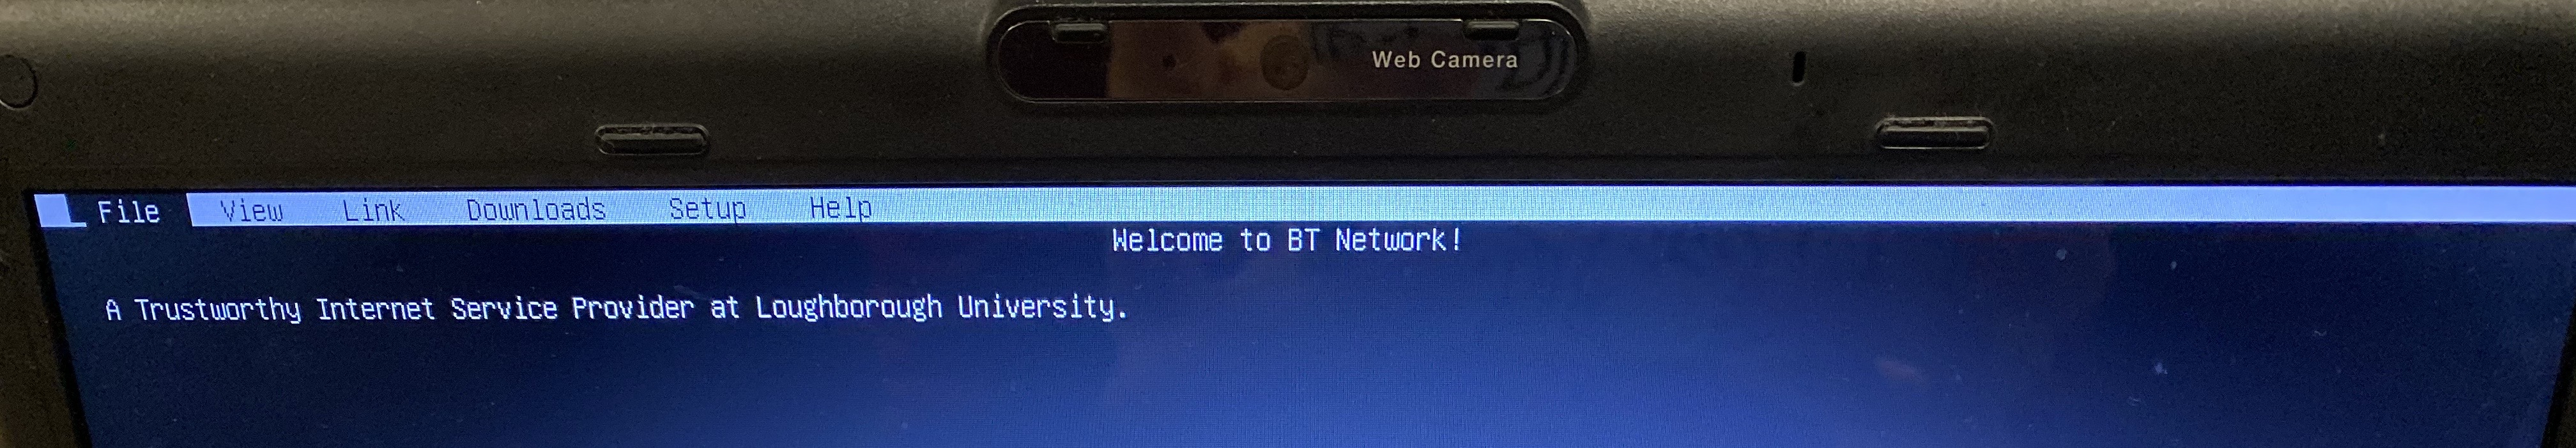
\includegraphics[width=\linewidth]{web1}
    \caption{Web Service Provided at \texttt{http://bt.lboro} .}
    \label{fig:web1}
\end{figure}




